\section{Evaluations}

\begin{table}
\caption{Spectulative Attack Results}
\label{tab:spec-attack-results}
\begin{tabular}{@{} *4l @{}} \toprule
    &                        & \multicolumn{2}{l}{Bytes per Second} \\
    Attack                  & Cycles for Secret Byte &           100MHz &   3.2GHz \\ \midrule
    Bounds Check Bypass     &                ~884485 &          113 bps & 3618 bps \\
    Branch Target Injection &                ~876602 &          114 bps & 3650 bps \\ \bottomrule
\end{tabular}
\end{table}

\begin{table}
\caption{BOOM Core Parameters}
\label{tab:boom-core-params}
\begin{tabular}{@{} *2l @{}} \toprule
    Parameter                    & Value \\ \midrule
    Fetch Width                  & 2 \\
    Decode Width                 & 2 \\
    Issue Width                  & 4 \\
    ROB Size                     & 100 \\ \midrule
    L1 Sets                      & 64 \\
    L1 Ways                      & 8 \\
    L1 Linesize                  & 64 bytes \\ \midrule
    BTB Sets                     & 512 \\
    BTB Banks                    & 2 \\
    BTB Ways                     & 4 \\ \midrule
    GShare History Bits          & 23 \\
    GShare Counter Table Entries & 4096 \\ \bottomrule
\end{tabular}
\end{table}

\begin{table}
\caption{Attack Parameters}
\label{tab:attack-params}
\begin{tabular}{@{} *2l @{}} \toprule
    Parameter                    & Value \\ \midrule
    Cache Hit Threshold          & 50 cycles \\
    Amount of runs on same byte  & 10 rounds \\
    Training rounds for BPU      & 6 training rounds \\
    Cache flush hits on same set & 4 * L1\_WAYS \\
    GShare Counter Table Entries & 4096 \\ \bottomrule
\end{tabular}
\end{table}

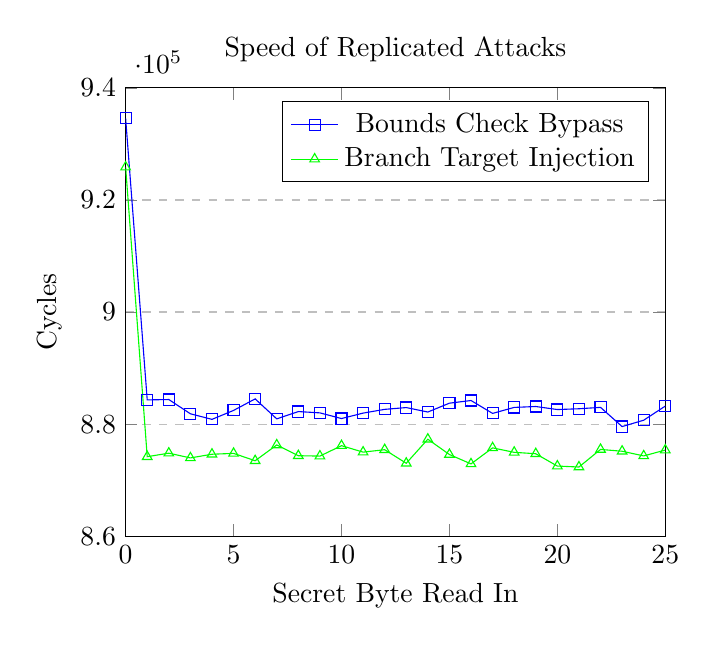
\begin{tikzpicture}
\begin{axis}[
    title={Speed of Replicated Attacks},
    ylabel={Cycles},
    xlabel={Secret Byte Read In},
    xmin=0, xmax=25,
    ymin=860000, ymax=940000,
    legend pos=north east,
    ymajorgrids=true,
    grid style=dashed
]

\addplot[
    color=blue,
    mark=square,
]
coordinates {
    (0 ,934580)
    (1 ,884322)
    (2 ,884387)
    (3 ,881845)
    (4 ,880847)
    (5 ,882446)
    (6 ,884498)
    (7 ,880939)
    (8 ,882241)
    (9 ,882006)
    (10,880994)
    (11,881965)
    (12,882634)
    (13,882954)
    (14,882156)
    (15,883738)
    (16,884212)
    (17,881912)
    (18,882980)
    (19,883142)
    (20,882600)
    (21,882739)
    (22,882989)
    (23,879563)
    (24,880698)
    (25,883218)
};
        
\addplot[
    color=green,
    mark=triangle,
]
coordinates {
    (0 ,925862)
    (1 ,874188)
    (2 ,874815)
    (3 ,873968)
    (4 ,874626)
    (5 ,874778)
    (6 ,873466)
    (7 ,876281)
    (8 ,874361)
    (9 ,874297)
    (10,876153)
    (11,875000)
    (12,875435)
    (13,873015)
    (14,877303)
    (15,874572)
    (16,872902)
    (17,875761)
    (18,874966)
    (19,874715)
    (20,872514)
    (21,872346)
    (22,875481)
    (23,875161)
    (24,874325)
    (25,875371)
};
\legend{Bounds Check Bypass,Branch Target Injection}

\end{axis}
\end{tikzpicture}

\subsection{Base Core Parameters}

The two different attacks were replicated on the BOOM core with the parameters given
in \ref{tab:boom-core-params}. All attacks were measured using FireSim, an open-source
cycle-accurate, FPGA-accelerated scale-out computer system simulation platform.

\subsection{Replicating Speculative Attacks}

Overall results of the replications are promising with \ref{tab:spec-attack-results}
showing the result of the two respective attacks. The cycle times were measured from
before the tally array clear to right before the printf of the results. Thus, this
measurement takes into account the clearing of the tally array before each run, the
multiple rounds of training for the BPU, the single attack run on the victim, and the
time to probe the attacker array. The results are close to each other because the code
shares similar structure. The main differences are around the setup of the fdiv manipulation
and the extra arithmatic in the Branch Target Injection case where you have to calculate
both the index and the address to pass into the function. 

\subsection{Spec Buffer}
